\documentclass[DM,lsstdraft,authoryear,toc]{lsstdoc}
\input{meta}

% Package imports go here.
\usepackage{listings}
\lstset{
basicstyle=\small\ttfamily,
columns=flexible,
breaklines=true
}
\usepackage{lscape}
\usepackage{makecell}


% Local commands go here.

%If you want glossaries
%\input{aglossary.tex}
%\makeglossaries

\title{ObsLocTap: Publishing the Rubin Observing Schedule}

% Optional subtitle
% \setDocSubtitle{A subtitle}

\author{%
William O'Mullane
}

\setDocRef{DMTN-263}
\setDocUpstreamLocation{\url{https://github.com/lsst-dm/dmtn-263}}

\date{\vcsDate}

% Optional: name of the document's curator
% \setDocCurator{The Curator of this Document}

\setDocAbstract{%
We are required to publish the Rubin observing schedule some hours in advance.  Following our VO fist strategy  IVOA ObsLocTap is a suitable protocol for doing this. The required  information is available from the scheduler and already in the EFD.
}

% Change history defined here.
% Order: oldest first.
% Fields: VERSION, DATE, DESCRIPTION, OWNER NAME.
% See LPM-51 for version number policy.
\setDocChangeRecord{%
  \addtohist{1}{YYYY-MM-DD}{Unreleased.}{William O'Mullane}
}


\begin{document}

% Create the title page.
%\maketitle
% Frequently for a technote we do not want a title page  uncomment this to remove the title page and changelog.
\mkshorttitle

\section{Introduction}
We are required to publish the observing schedule and choose ObsLocTap\footnote{\url{documents/ObsLocTap}} as the protocol.



\section{Implementation}

There are two parts to this implementation:

\begin{enumerate}
\item The postgress database and populating it.
\item Serving that up via TAP.
\end{enumerate}


No 2. here is well understood  - we have TAP services so we put one in front of the \DB

There are some choices to be made concerning No. 1.

Frossie provided the simple diagram \figref{fig:obsloctap} which captures the ideas.


\begin{figure}
\begin{centering}
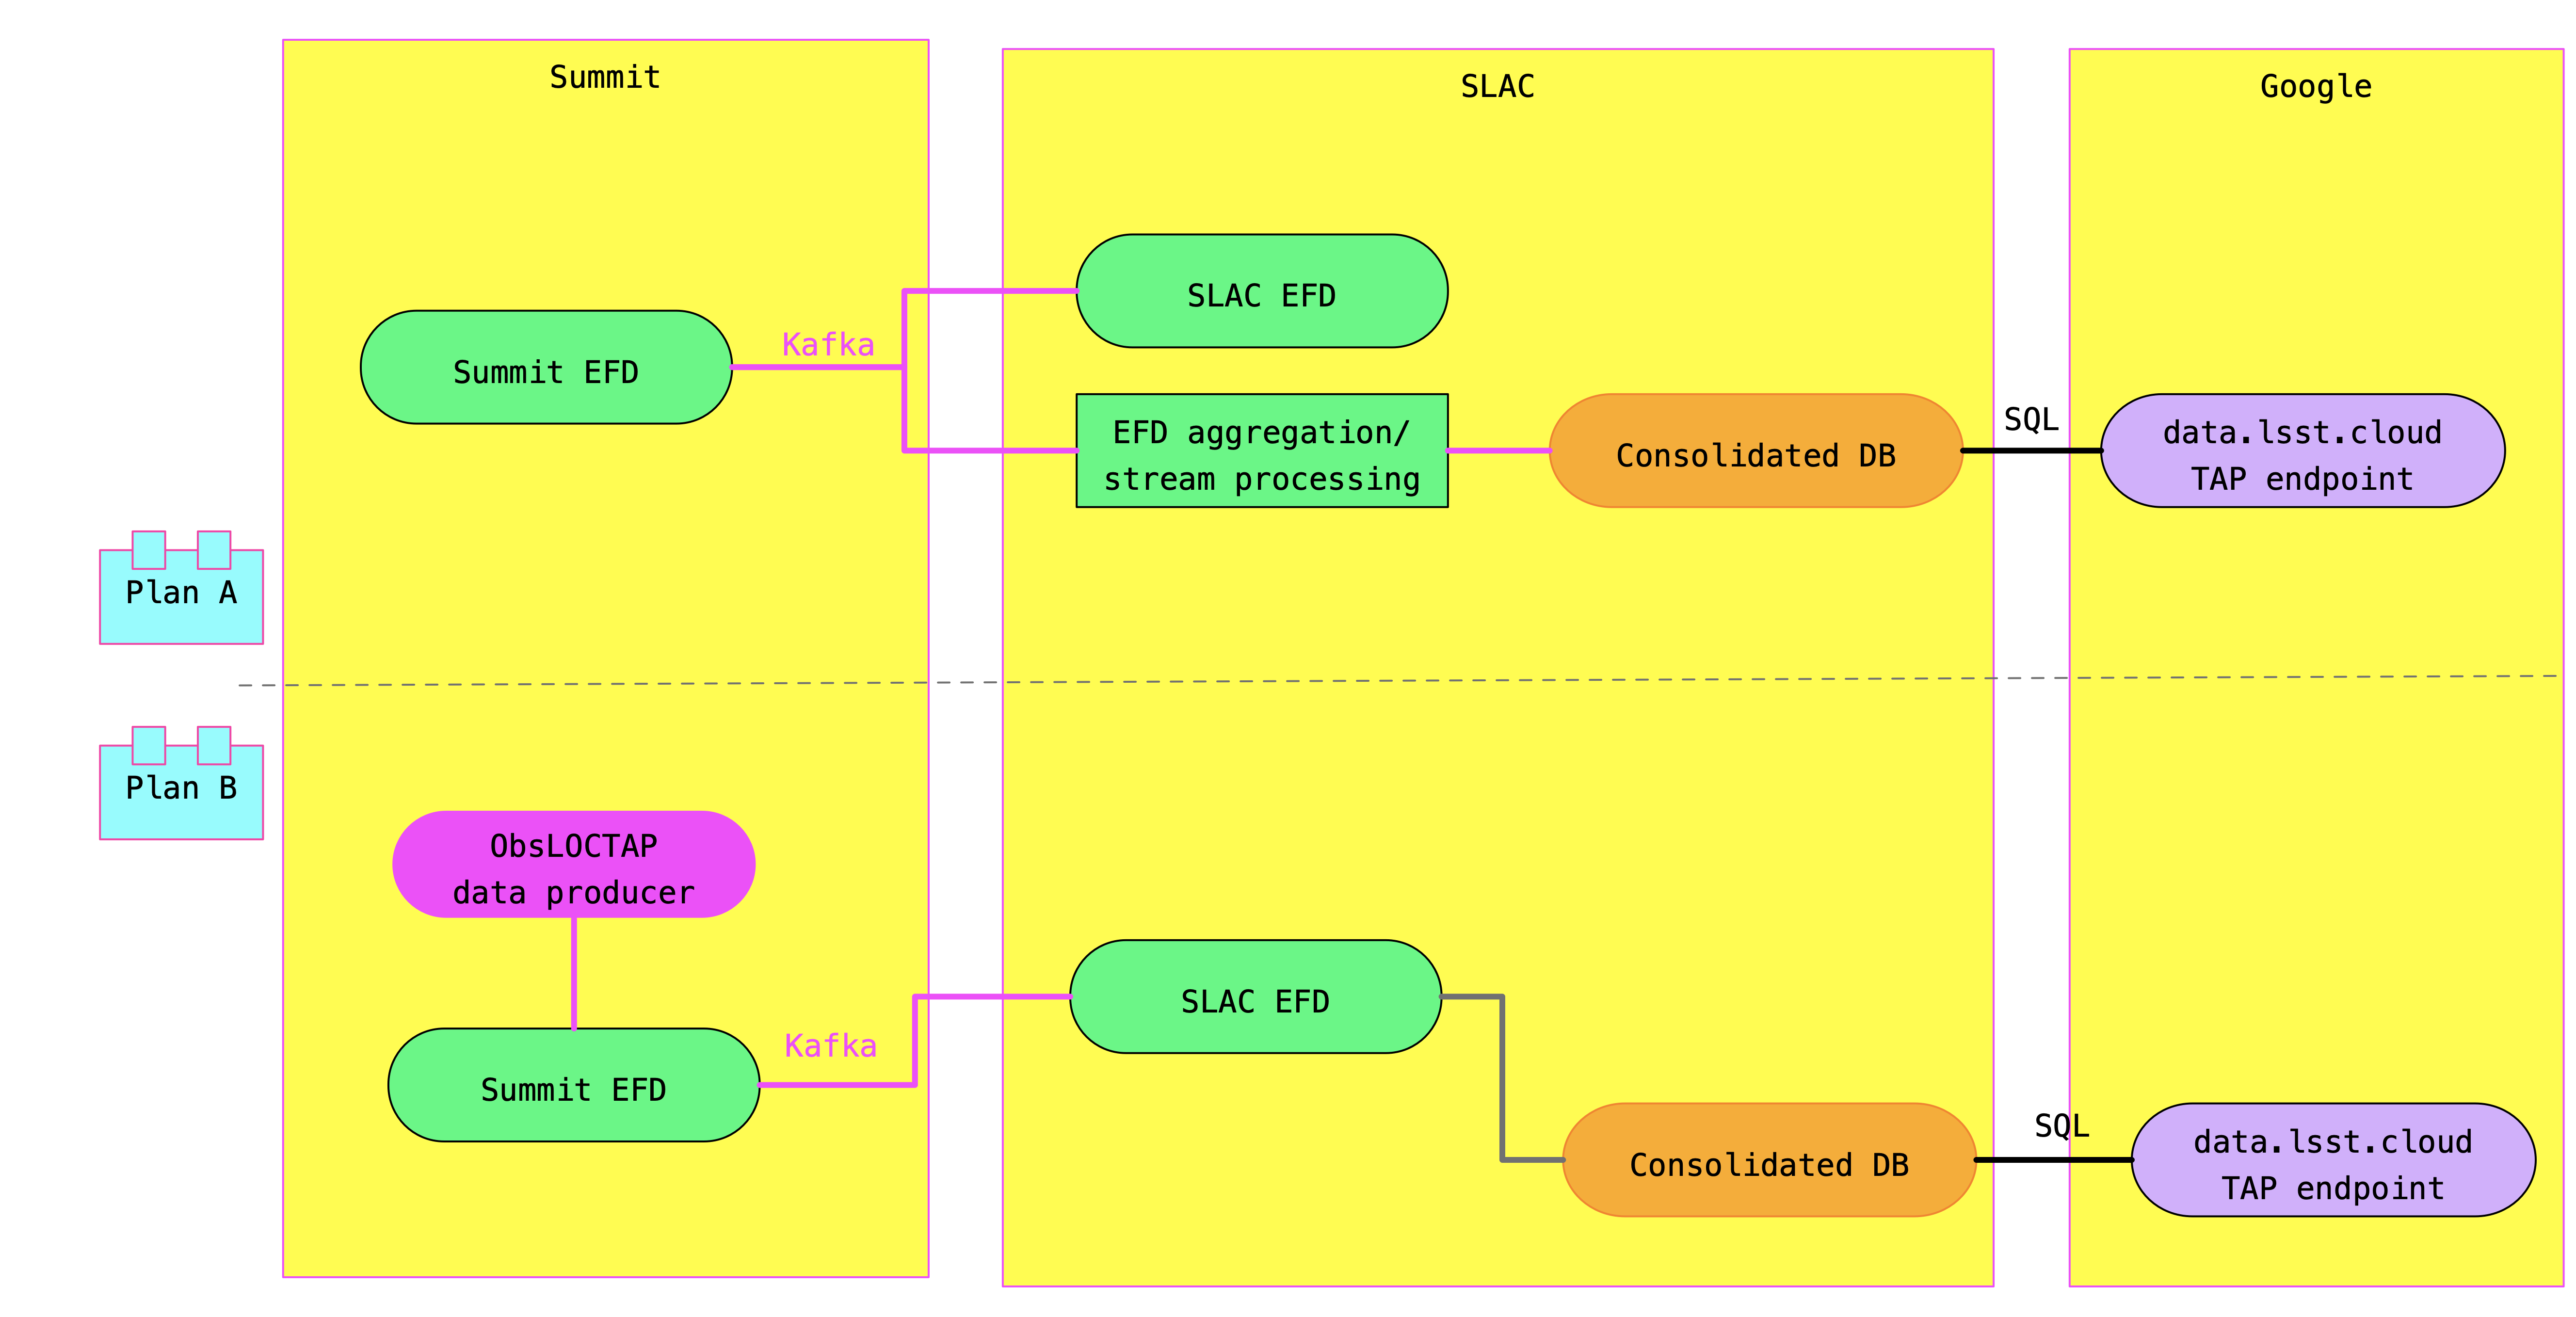
\includegraphics[width=0.8\textwidth]{obsloctap}
	\caption{ Choices on how to populate the postgress database for ObsLocTap.
\label{fig:obsloctap}}
\end{centering}
\end{figure}


\subsection{Create the table}
The schems was added to {\code sdm\_schema} so felis may be use dto cerate the schema.

I did not find felis on pips so I grabbed \url{git@github.com:lsst/felis.git} and installed it with {\tt pip install .}.

I also cloned \url{git@github.com:lsst/sdm_schemas.git}.

This allowed the felis executioni, database login and table creation:i\footnote{ivoa. was removed  from th DDL} \\
\begin{code}
felis create-all --engine-url="\$engine\_url" --dry-run  sdm\_schemas/yml/obsloctap.yaml > obsloctap.sql

psql -h usdf-butler-session.slac.stanford.edu -U rubin lsstdb1

lsstdb1=> create schema obsloctap;
lsstdb1=> create schema obsloctap\_dev;

SET SEARCH_PATH = obsloctap_dev;
\i obsloctap.sql
SET SEARCH_PATH = obsloctap;
\i obsloctap.sql
\end{code}




\subsection{Populating the \DB}

Initially at least we should try plan A and do all of this at the USDF.
The EFD messages are replicated there so we can pick up the scheduler messages and process them via a stream processor in Kafka (within Sasquatch).

The 24 hour schedule should probably get a new topic to make it distinct from the normal operations - this has to be agreed with scheduler/summit. This will be processed to create schedule entries.

Then we will process {\texttt lsst.sal.Scheduler.logevent\_predictedSchedule } to update/create schedule entries.

Finally we will look at {\texttt lsst.sal.ATHeaderService.logevent\_largeFileObjectAvailable} which will give us a pointer to the header ({\texttt url} field) and using {\texttt astro\_metadata\_translator}  we can get r obsid, exposure\_id, filter and update the \DB appropriately.

\subsection{TAP service}

There is already a ticket \jira{DM-39729} for the creation of the Felis schema.
Another is needed to expose this via tap.

Along the lines of separation of security concerns this would be deployed on the Cloud (US DAC) not in USDF.


\appendix
\section{Obsplan table from ObsLocTap} \label{sec:obsplan}
%This is copied from https://www.ivoa.net/documents/ObsLocTAP/20210724/REC-ObsLocTAP-1.0-20210724.tex

The obpsplan tabel schema from the "Observation Locator Table Access Protocol
Version 1.0" is provided here for ease of reference.

\begin{landscape}
\begin{table}
\def\hlstrut{\vrule height 13pt depth5pt width0pt}
\begin{tabular}{ |l|l|l| }
\hline
\hlstrut\textbf{Column Name} &
\hlstrut\textbf{Description} &
\hlstrut\textbf{Constraint} \\
\hline
%row no:2
t\_planning &
Time in MJD when this observation has been added or modified into the
planning log &
not null\\
\hline
%row no:3
target\_name &
Astronomical object observed, if any &
\\
\hline
%row no:4
obs\_id &
Observation ID &
not null\\
\hline
%row no:5
obs\_collection &
Name of the data collection &
\\
\hline
%row no:6
s\_ra &
Central right ascension, ICRS &
\\
\hline
%row no:7
s\_dec &
Central declination, ICRS &
\\
\hline
%row no:8
s\_fov  &
Diameter (bounds) of the covered region &
\\
\hline
%row no:9
s\_region &
Sky region covered by the data product (expressed in ICRS frame) &
\\
\hline
%row no:10
s\_resolution &
Spatial resolution of data as FWHM &
\\
\hline
%row no:11
t\_min &
Start time in MJD &
\makecell[l]{not null for execution\_status \\ Scheduled or Performed} \\
\hline
%row no:12
t\_max &
Stop time in MJD &
\makecell[l]{not null for execution\_status \\ Scheduled or Performed} \\
\hline
%row no:13
t\_exptime &
Total exposure time &
\makecell[l]{not null for execution\_status \\ Scheduled or Performed} \\
\hline
%row no:14
t\_resolution &
Temporal resolution FWHM &
\\
\hline
%row no:15
em\_min &
Start in spectral coordinates &
\\
\hline
%row no:16
em\_max &
Stop in spectral coordinates &
\\
\hline
%row no:17
em\_res\_power &
Spectral resolving power &
\\
\hline
%row no:18
o\_ucd &
UCD of observable (e.g., phot.flux.density, phot.count, etc.) &
\\
\hline
%row no:19
pol\_states &
List of polarization states or NULL if not applicable &
\\
\hline
%row no:20
pol\_xel &
Number of polarization samples &
\\
\hline
%row no:21
facility\_name &
Name of the facility used for this observation &
not null\\
\hline
%row no:22
instrument\_name &
Name of the instrument used for this observation &
\\
\hline
%row no:23
t\_plan\_exptime &
Planned or scheduled exposure time &
\\
\hline
%row no:24
category &
Observation category. One of the following values: Fixed, Coordinated, Window,
Other &
not null\\
\hline
%row no:25
priority &
Priority level $ \{ $ 0, 1, 2$ \} $ &
not null\\
\hline
%row no:26
execution\_status &
One of the following values:  Planned, Scheduled, Unscheduled, Performed, Aborted &
not null\\
\hline
%row no:27
tracking\_type &
One of the following values:  Sidereal, Solar-system-object-tracking,
Fixed-az-el-transit &
not null\\
\hline
\end{tabular}
\caption{ObsPlan columns description}
\label{tab:obsplancolumns}
\end{table}
\end{landscape}

% Include all the relevant bib files.
% https://lsst-texmf.lsst.io/lsstdoc.html#bibliographies
\section{References} \label{sec:bib}
\renewcommand{\refname}{} % Suppress default Bibliography section
\bibliography{local,lsst,refs_ads,refs,ivoa}

% Make sure lsst-texmf/bin/generateAcronyms.py is in your path
\section{Acronyms} \label{sec:acronyms}
\addtocounter{table}{-1}
\begin{longtable}{p{0.145\textwidth}p{0.8\textwidth}}\hline
\textbf{Acronym} & \textbf{Description}  \\\hline

API & Application Programming Interface \\\hline
CADC & Canadian Astronomy Data Centre \\\hline
DAC & Data Access Center \\\hline
DB & DataBase \\\hline
DESC & Dark Energy Science Collaboration \\\hline
DM & Data Management \\\hline
DMS & Data Management Subsystem \\\hline
DMS-REQ & Data Management System Requirements prefix \\\hline
DMSR & DM System Requirements; LSE-61 \\\hline
DMTN & DM Technical Note \\\hline
EFD & Engineering and Facility Database \\\hline
FWHM & Full Width at Half-Maximum \\\hline
ICRS & International Celestial Reference Frame \\\hline
IVOA & International Virtual-Observatory Alliance \\\hline
JSON & JavaScript Object Notation \\\hline
LCR & LSST Change Request \\\hline
LSE & LSST Systems Engineering (Document Handle) \\\hline
MJD & Modified Julian Date (to be avoided; see also JD) \\\hline
OCS & Observatory Control System \\\hline
OSS & Observatory System Specifications; LSE-30 \\\hline
SAL & Service Abstraction Layer \\\hline
SQL & Structured Query Language \\\hline
TAP & Table Access Protocol \\\hline
UCD & Unified Content Descriptor \\\hline
US & United States \\\hline
USDF & United States Data Facility \\\hline
VO & Virtual Observatory \\\hline
\end{longtable}

% If you want glossary uncomment below -- comment out the two lines above
%\printglossaries





\end{document}
